
\documentclass[11pt, letterpaper]{article}
\usepackage{cite}
\usepackage{geometry}
\usepackage{graphicx}
\usepackage{subcaption}
\usepackage{wrapfig}

\geometry{margin={1.00in, 1.00in}}

\title{Tracking Global Spread of Disease through Air Travel}
\author{Sean Brennan, Henry Kautz, Adam Sadilek}
\date{Dec. 18, 2012}

\begin{document}
    \maketitle

    \section{Introduction}
        \subsection{Problem Statement}
            In this project, we leveraged data mining and machine learning techniques to track the global spread of disease via airports and air travel. This project built upon a combination of past techniques devised by Adam Sadilek et al to accurately identify indicators of illness in geotagged tweets, as well as some degree of geospatial inference to discover who was tweeting from an airport. Additionally, this project involved a novel probabilistic model for user encounters, which we hoped would improve our system's classification and predictive abilities. We discuss these methods and our results in more detail in the coming sections.

        \subsection{Problem Importance}
            It is no secret that air travel can increase your risk of falling ill: flying it is a system that forces you to be in a tight and poorly ventilated space with dozens or even hundreds of strangers. This is not even taking factors such as jet lag and other forms of travel fatigue into account, both of which can make you vulnerable to or exacerbate otherwise insignificant ailments. These issues, combined with the rise of affordable mass transit in the previous century, have completely changed the spatial and temporal scopes of epidemiology. People are now able to travel much farther and faster than anyone could have imagined 100 years ago. The SARS epidemics of 2002 and 2003 are salient examples of how disease can propagate through this global transit network like wildfire.

            \begin{figure}[b!]
                \begin{center}
                    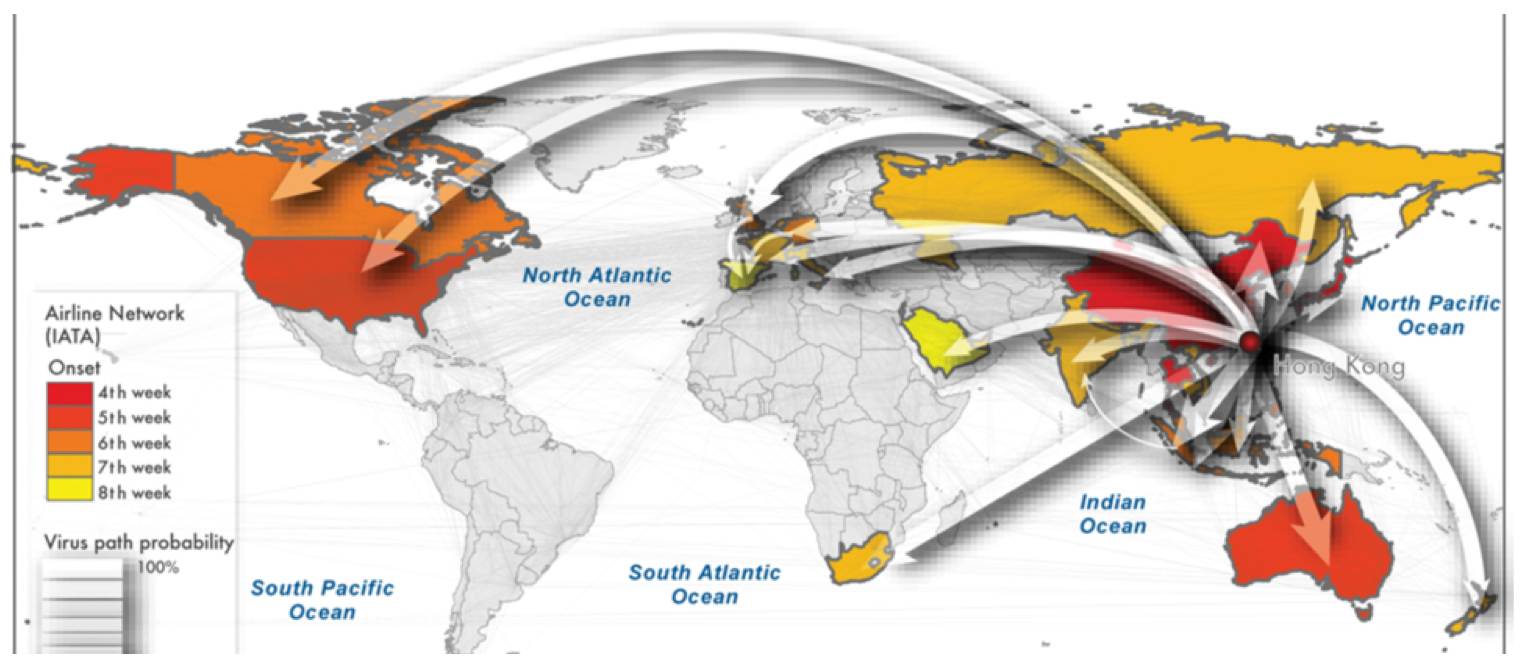
\includegraphics[width=0.75\textwidth]{sars-example.png}
                    \caption{Map showing the rapid propagation of SARS over the globe. \cite{colizza}}
                    \label{meetings-example}
                \end{center}
            \end{figure}

        \subsection{Background \& Related Work}
            Though people have been aware of the increased risk of disease transmission on commercial planes for a long time, the effect was first studied in depth in 1979. In a seminal case study, passengers that were stuck aboard a plane delayed for three hours were found to have an incredibly high incidence of influenza within 72 hours of landing. This was an especially dramatic example since there was only one passenger aboard initially who had influenza. \cite{moser} Similar results were found in 2009, at the height of the H1N1 influenza scare. In a case study of two flights to Australia in this time frame, even just 2\% of passengers having some influenza-like illness increased the post-flight incidence rate of influenza to 5\%. In addition, it was found that sitting within 2 seats of a passenger with influenza would increase the likelihood of you contracting influenza to almost 8\%. \cite{foxwell}

            However, a major hurdle in this line of study that impedes effective response to these crises is modeling the new ways in which humans travel in the 21st century. In past eras, the spread of disease could be modeled as a fairly intuitive and smooth spatial diffusion phenomenon. The bubonic plague's course over Europe is a classic example of this, in that it would travel somewhere around 200 miles a year in every direction. \cite{colizza} However, with the convenience of air travel, this smooth diffusion is now intermingled with short periods of very fast travel over long distances, yet many epidemiological models do not account for this so-called ``super-diffusive'' movement. \cite{brockmann} Another serious difficulty is finding these patterns at population scale. Even just a decade ago, it was either infeasible or completely impossible to study epidemiological phenomena at such a huge scale in a time frame as short as a week.

            Fortunately, there is now a solution: social media sites such as Twitter give us a unique opportunity to witness crowd movement and interaction in real time and at population scale. As such, I would be remiss to not mention the work that we have done related to inferring sickness from Twitter data. Our approach is a semi-supervised one and involves training two support vector machines over a huge corpus of tweets. One SVM is heavily penalized for false positives and thus becomes very good at positively identifying sick tweets; the other is heavily penalized for false negatives and thus becomes very good at identifying tweets that are not about sickness. This approach is beneficial because of the serious class imbalance issues: there are millions of tweets per hour, but only an infinitesimal amount of them are relevant to a user's health state. Training data for these SVMs was gathered by having users on Amazon's Mechanical Turk label the initial set as ``sick'' or ``other''. \cite{sadilek}

    \section{Methodology}
        \subsection{Data Acquisition}
            Data was acquired primarily through harvesting geotagged tweets via Twitter's Search API over a period of several weeks. The Search API is powerful in that it enables users to pull in a huge volume of recent tweets, and it allows you to build very specific and precise queries for finding exactly the data you are looking for. I used the Search API's powerful bounding box query capabilities to find tweets only within a three kilometer radius of the 100 most trafficked airports in the United States. I only concerned myself with tweets in the English language, since this is the only language our classifiers learned words and phrases for.

            After a week or so of collecting this initial data set, we began to supplement our broad knowledge of what was occurring within airports with deep knowledge of particular users' histories. We started by looking for users who had, according to our data, tweeted from more than one airport. This ended up being approximately 20\% of users in our database. As these users were identified, we queued them to have 100 of their latest tweets pulled from their timeline via Twitter's REST API. The goal behind this collection was to attempt to uncover these users' health states before, after, and in between tweets made from airports. It is critical to have this information because sometimes users, for example, tweet about being sick, then go to the airport and tweet something unrelated to their health state. Furthermore, these ``frequent flyers'' are the ligature of our network: they are the highly ranked users who are the most likely to encounter the most people. Therefore, if they are sick, their individual health risks will have the greatest impact on the network at large.

        \subsection{Algorithms}
            \subsubsection{Classification}
                The fundamental approach that defined our earlier work is still at the heart of this new branch of research: Adam's support vector machine algorithm for classifying sick and healthy individuals. The SVMs learned weights for sequences of up to three words; these weights were then used to calculate some aggregate score for all trigrams in the tweet. We used this classification to obtain the initial health rating of each individual tweet. For more detailed information on how this works, please consult Adam's paper on the subject. \cite{sadilek}

                \begin{wrapfigure}{r}{0.5\textwidth}
                    \begin{center}
                        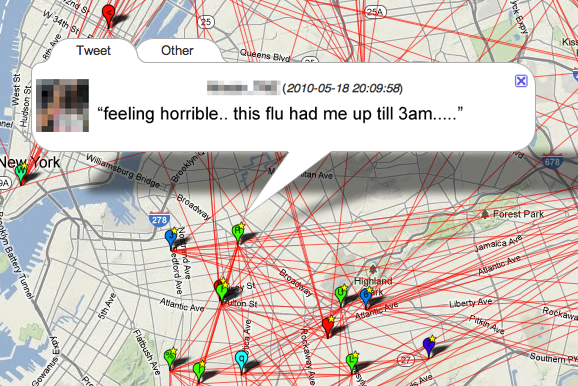
\includegraphics[width=0.5\textwidth]{meetings-example.png}
                        \caption{A conceptual example of how one sick user can affect those around her.}
                        \label{meetings-example}
                    \end{center}
                \end{wrapfigure}

                However, this foundational work, though incredibly valuable and well-supported by official data, only scratches the surface of the problem. One issue is that it treats each tweet as an isolated observation in time and space. It does not account for how previous tweets might have bearing on this one - for example, had the user previously tweeted about being ill? It also considers health risk as something observable solely through what a user says about his or herself: the people who that user met do not enter the equation at all. This is an important detail because an individual can spread disease to others before becoming symptomatic and complaining about it on Twitter; even worse, an individual can transmit diseases to others without ever actually becoming sick with that disease.

                So clearly who you met has a bearing on your health risk. However, for the most part, these meetings are not directly observable. Therefore, we need a probabilistic graphical model of how these users interact. This model also needs to be temporal: it needs to recognize that a user's current health risk is some function of that user's previous health risk, as most diseases don't run their course that quickly. Finally, it needs to account for geospatial data as well, as you are most likely to have met other users who were observed as being close to your current location

            \subsubsection{Dynamic Bayesian Networks}
                \begin{figure}[t!]
                    \begin{center}
                        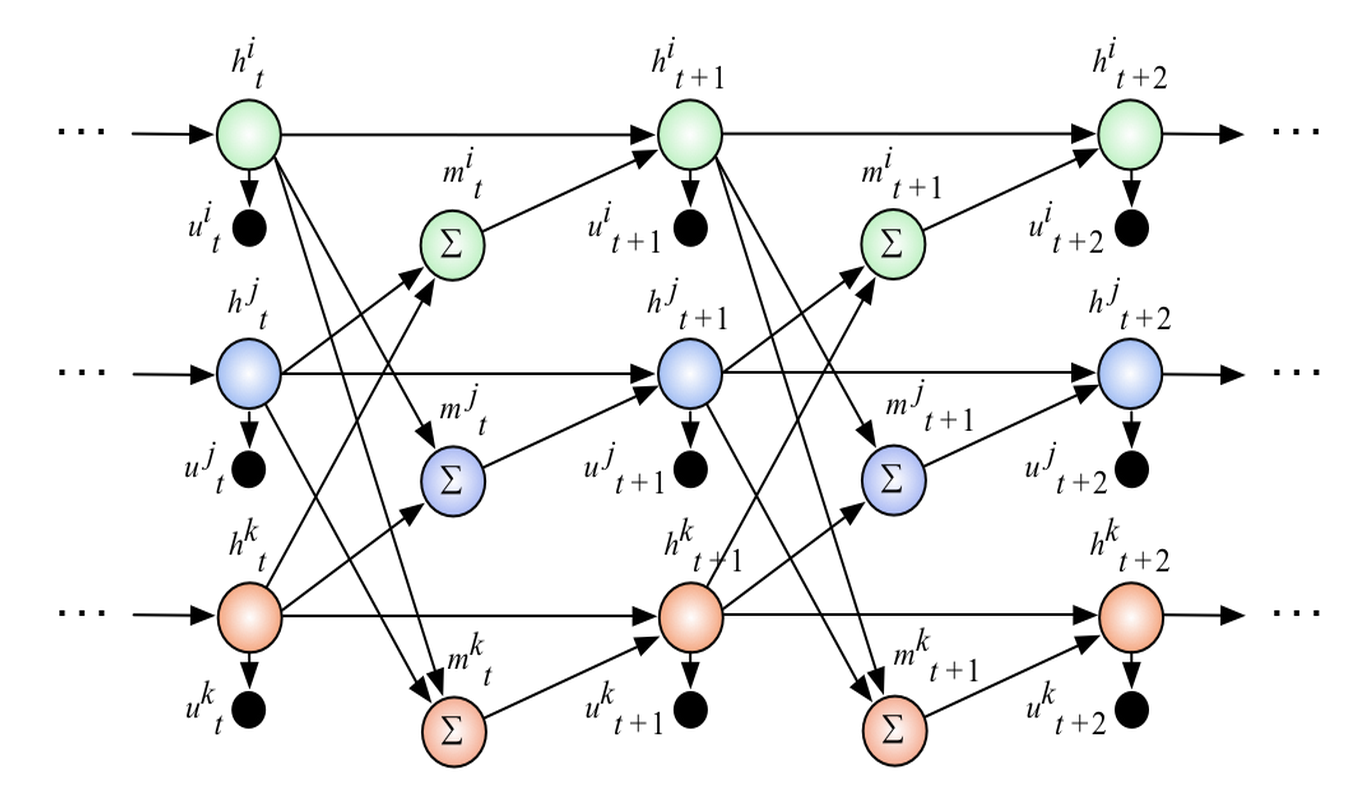
\includegraphics[width=1.0\textwidth]{dbn_example.png}
                        \caption{An example of a dynamic Bayesian network for our data set.}
                        \label{dbn-example}
                    \end{center}
                \end{figure}

                The graphical model that is most applicable to what I have just described is a dynamic Bayesian network. The primary distinction between a regular Bayes net and a DBN is that DBNs also perform Bayesian inference across adjacent time steps. In this way, they are also quite similar to Markov chains and hidden Markov models in that the initial probability for every vertex at each step is dependent only upon the probability at the previous step - this is the famous ``Markov property''.

                Our problem can be formulated very nicely into a dynamic Bayesian network, practically without any difficulty or effort. We used the Graphical Models Toolkit to create our DBNs, which is a freely available and open-source tool from the University of Washington. Each time step in the DBN represents an entire day, and every vertex within that time step represents a user.

                Each user vertex in a time slice can have an attached observation which represents their maximum health risk over that time frame; this information is acquired from our earlier classification of tweets. A user will not have a health risk observation at a certain time slice if they did not tweet at all during that time slice. Additionally, each user vertex in each time slice is ``pointed to'' by a meeting node. This meeting node represents a weighted sum of all health risks of all people you met in the previous time slice. Finally, every user vertex is ``pointed to'' by its corresponding vertex from the previous time slice.

                This model is no doubt easier to understand in picture form, so you can consult Figure~\ref{dbn-example} for a simple example DBN for our data set.

        \subsection{Feature Extraction}
            With our new formulation of meetings, nailing down the features that would define the DBN was absolutely critical. First there is the issue of when we should consider a user ``sick'' or ``healthy''. In the past, we have found that a score of 0.8 or above was a pretty good threshold that maximized positive examples and minimized noise. (By the way, due to our classification process, this score is not yet normalized - the normalized score would probably be around 0.75) It turned out to be an equally good threshold for this project.

            The truly problematic component in feature extraction was finding quality thresholds for meetings. In our model, meetings are considered to be undirected or rather bidirectional; that is, if two users have a meeting, both users' health scores affect one another. This means that, given $n$ users, the number of conceptually possible meetings per time slice is $O(n^2)$. Obviously, for populations in the tens of thousands of users, complexity of this magnitude is unacceptable. It's especially unacceptable when you consider that, even within the same time slice, it's highly unlikely that two users will ever meet. Keep in mind that meetings here represent some probability that a user infects another user: this requires pretty tight temporal and geospatial similarity. We have found that a time difference of 1 hour or less and a spatial difference of 100 meters or less has led to good performance.

    \section{Analysis}
        With such a large corpus of changes to our original project, there are certainly many new parameters to consider and analyze. Obviously, it is first worthwhile to discuss whether the machine learning approach to finding sick individuals is at all appropriate in the first place. Next, we must see if new features, such as backtracking over ``frequent flyers'' and our novel meetings model, increase the accuracy of our overall system. We accomplish both of these tasks by correlating the data we have collected and inferred with official statistics, specifically with Google Flu Trends. Google Flu Trends itself is a tried-and-true system that has been shown to correlate powerfully with official CDC data. More importantly, Google Flu Trends updates faster than the CDC, which allowed us to perform our analysis in a more timely manner. Finally, we will discuss our novel measure, disease influx, that we hope will allow us to foresee surges in sickness in geographic areas.

        \subsection{Regional Analysis}
            \begin{figure}[t!]
                \begin{center}
                    \begin{subfigure}[t]{0.45\textwidth}
                        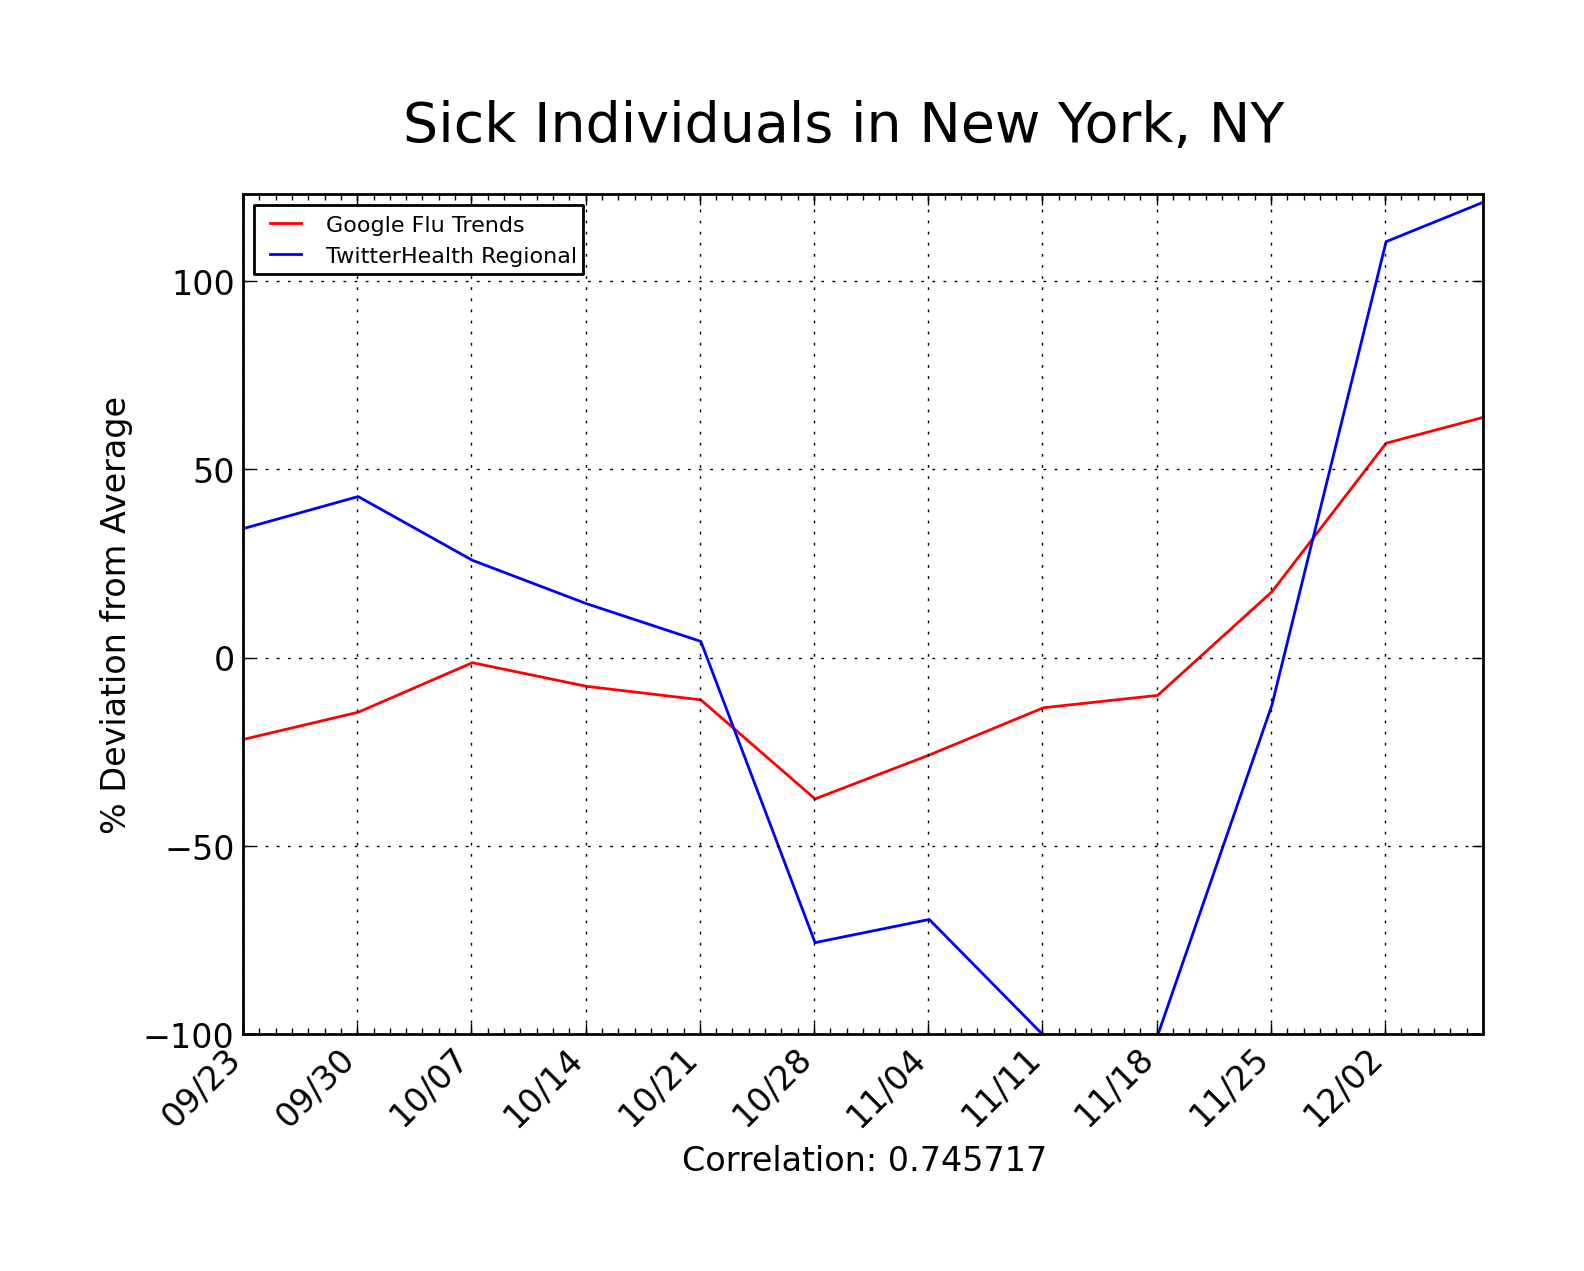
\includegraphics[width=\textwidth]{../plot/figures/NYC_mob_2012-12-15.png}
                    \end{subfigure}
                    \begin{subfigure}[t]{0.45\textwidth}
                        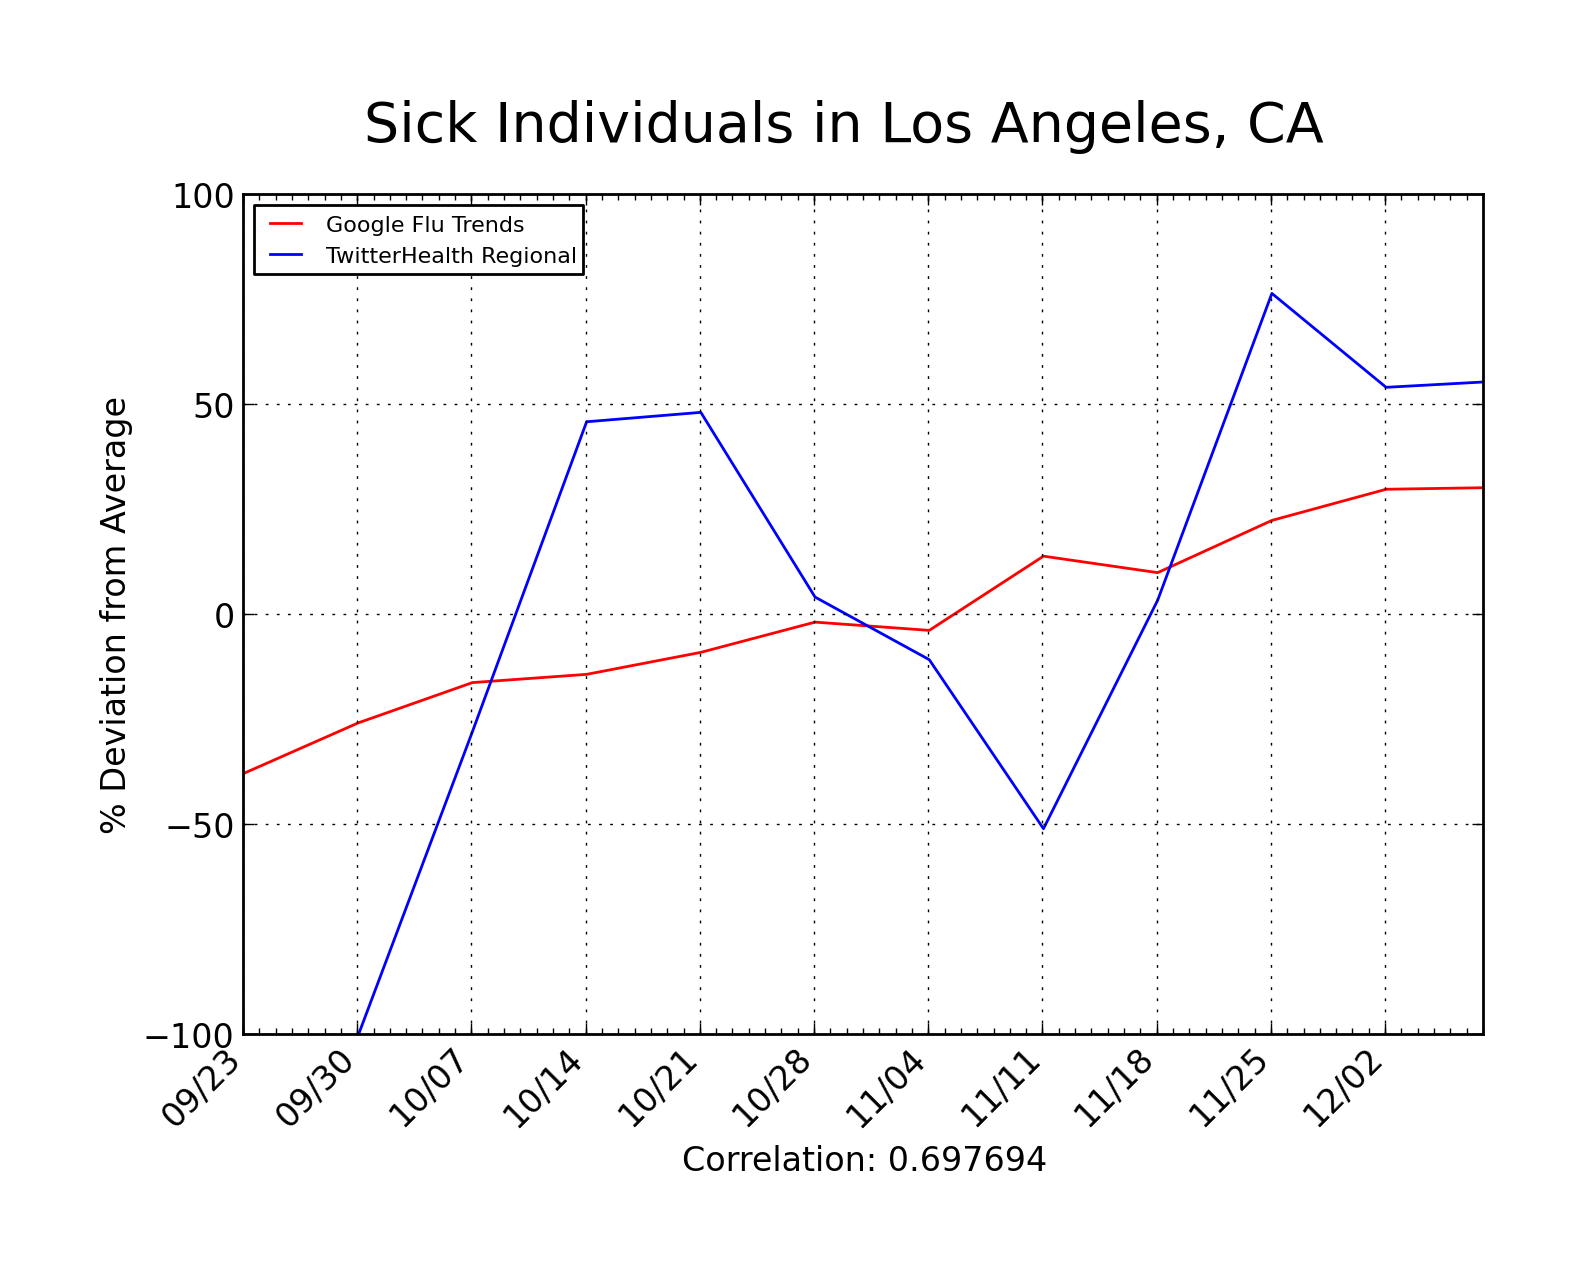
\includegraphics[width=\textwidth]{../plot/figures/LA_mob_2012-12-15.png}
                    \end{subfigure}
                    \begin{subfigure}[b]{0.45\textwidth}
                        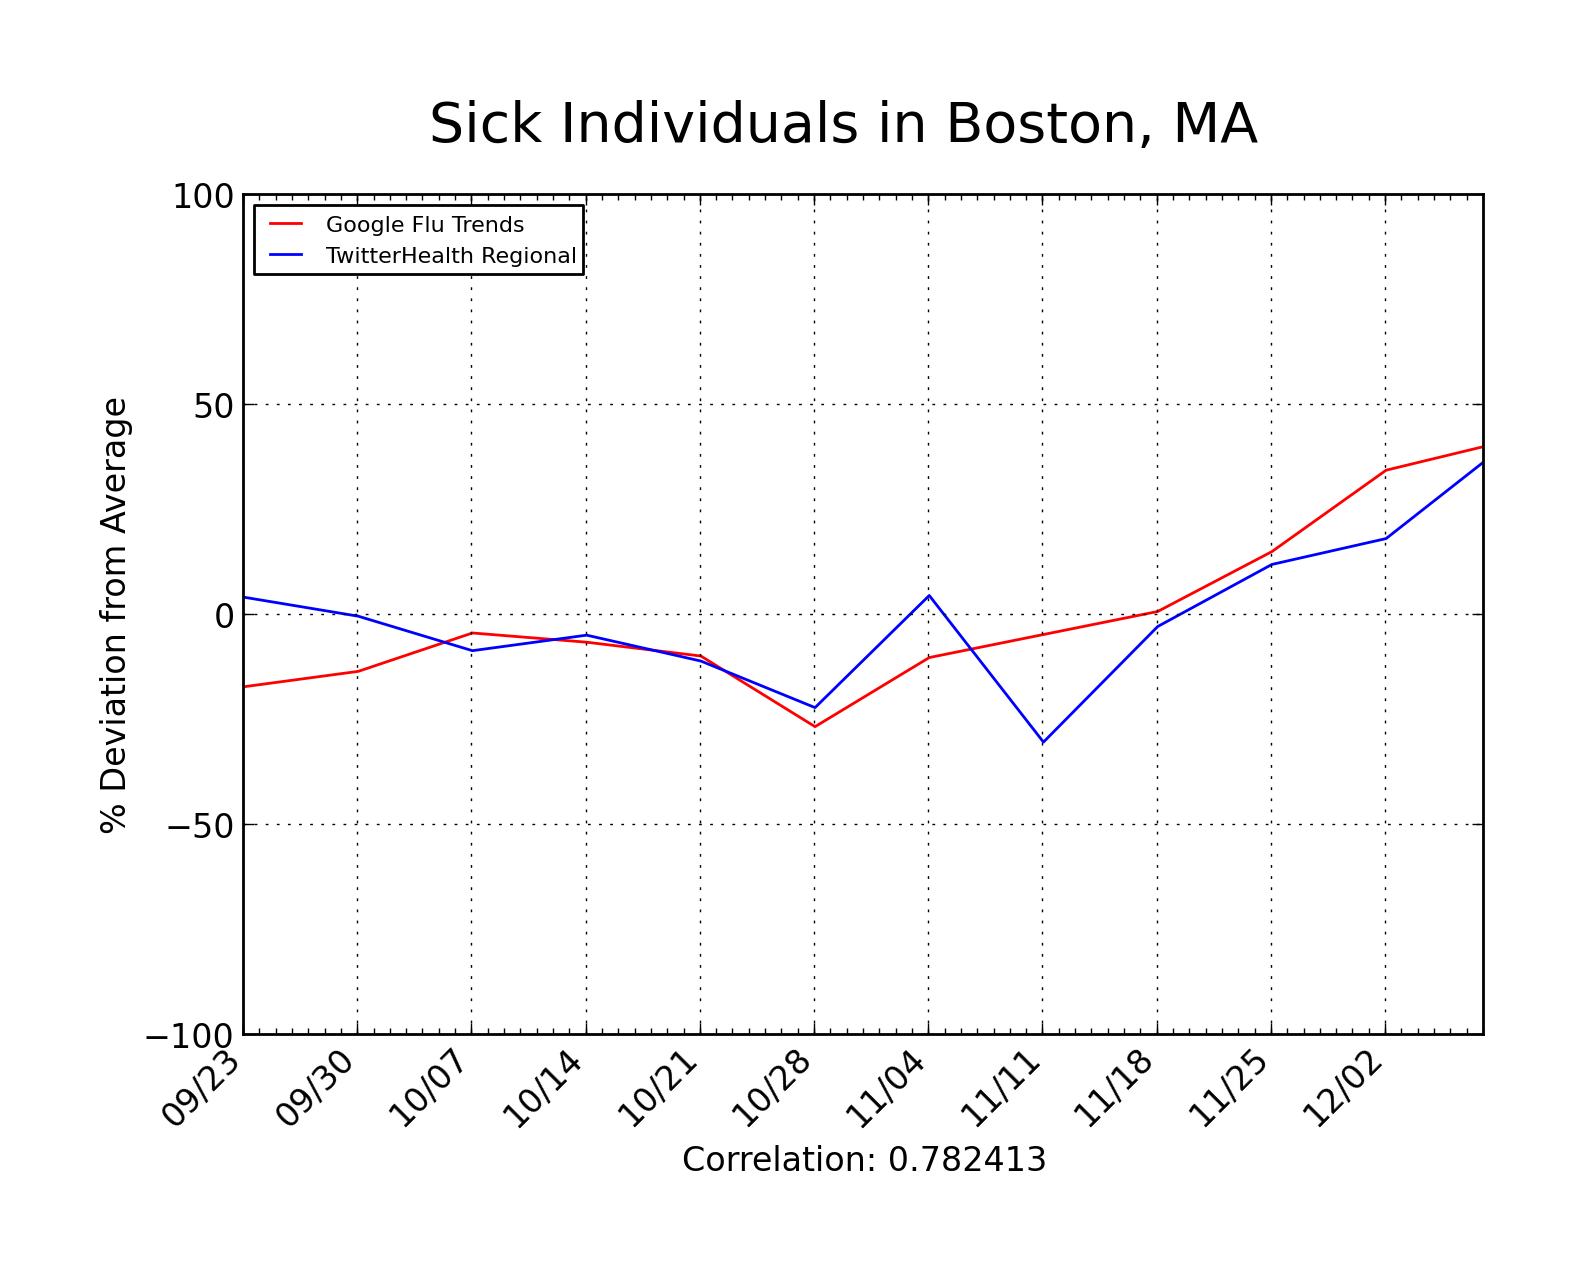
\includegraphics[width=\textwidth]{../plot/figures/BOS_mob_2012-12-15.png}
                    \end{subfigure}
                    \begin{subfigure}[b]{0.45\textwidth}
                        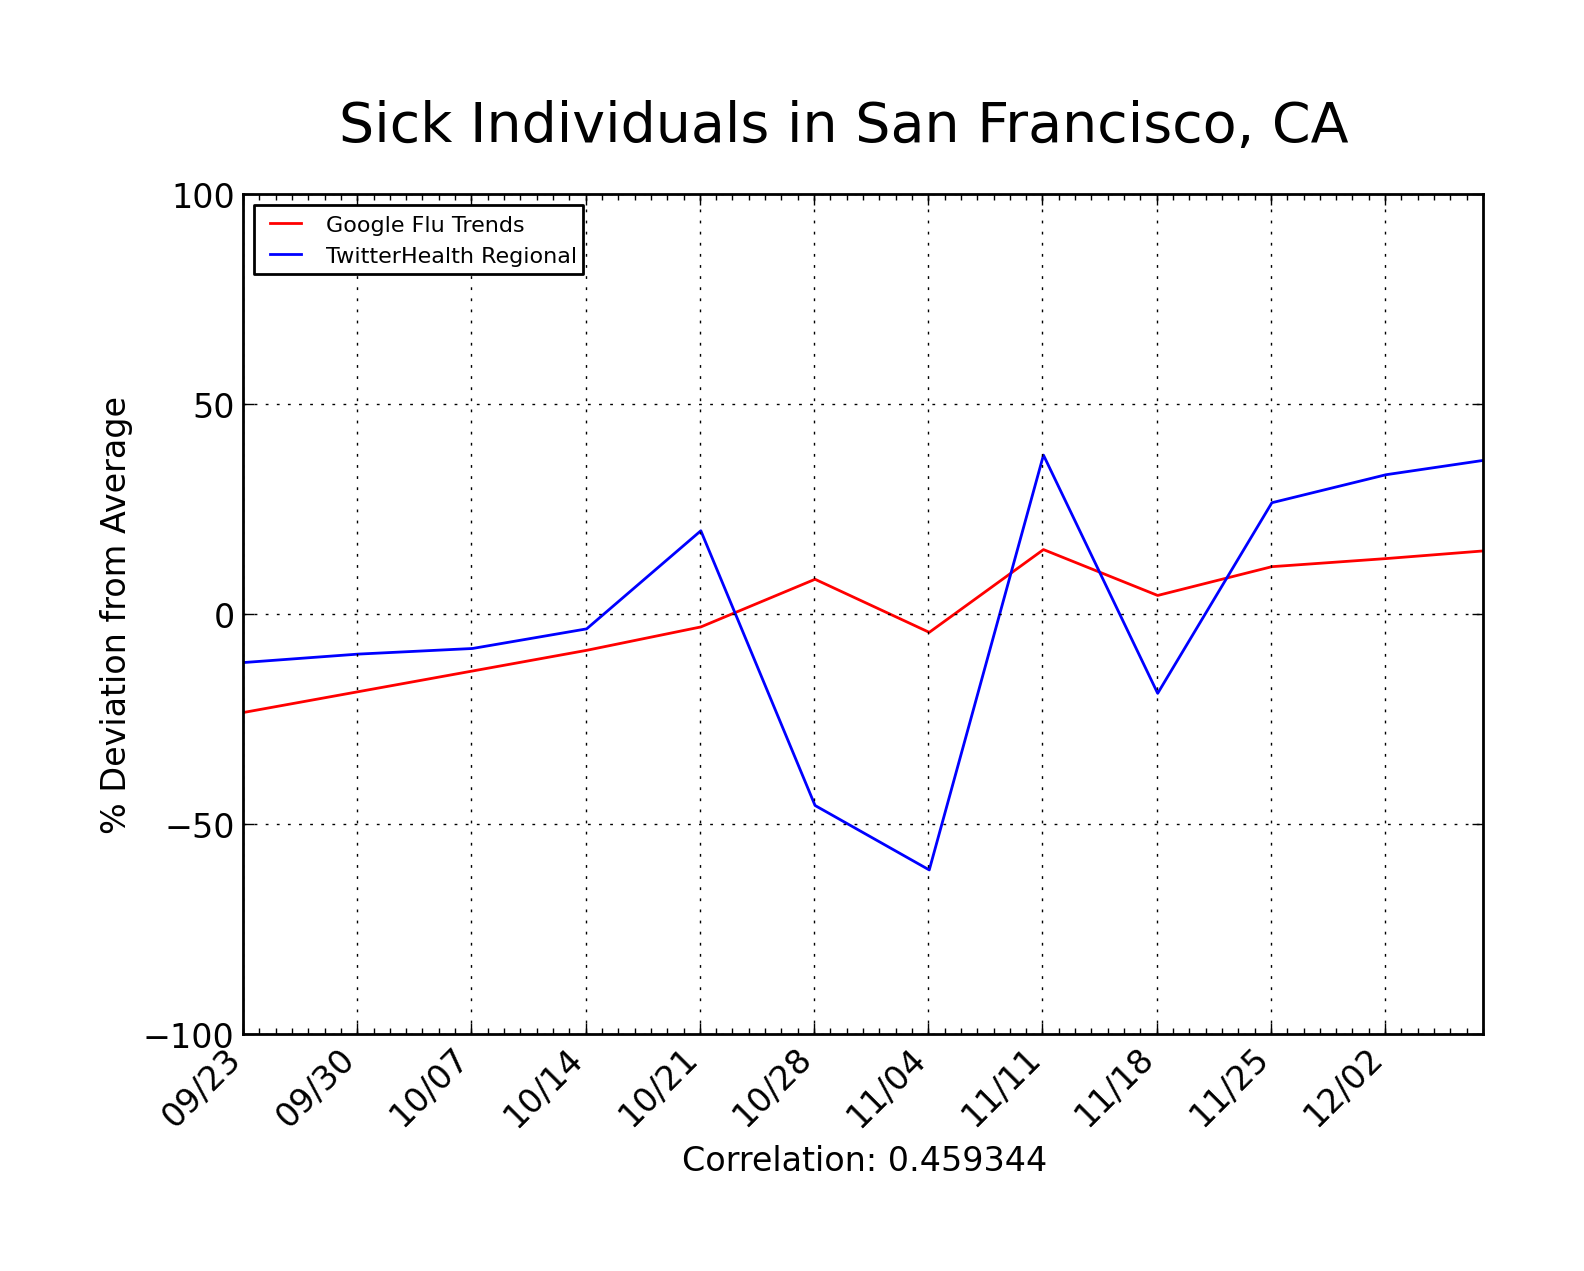
\includegraphics[width=\textwidth]{../plot/figures/SF_mob_2012-12-15.png}
                    \end{subfigure}
                    \caption{Regional results from previous datasets, and their correlations with Google Flu Trends data.}
                    \label{mobile-comparison}
                \end{center}
            \end{figure}

            The first bit of analysis we did was more of a sanity check than anything else. In the past we have collected massive data sets of tweets for large U.S. cities that we have classified as sick or healthy, so we wanted to see whether our classifications matched up with Google Flu Trends statistics. If our data showed no correlation or, even worse, a negative correlation, then obviously it was not worthwhile to try to build off our original scheme. Happily, this was not the case.

            In Figure~\ref{mobile-comparison}, you can see our data collected over the New York City, Los Angeles, Boston, and San Francisco metropolitan areas plotted against Google Flu Trends data for those same regions. We chose to plot the percent deviation from the average for each set rather than the actual number of sick individuals in each set because the Google Flu Trends dataset is far larger than ours. We also aggregated our data across weeks, because the Google Flu Trends data available to the public only comes in week intervals. This was much more meaningful, however, as scores can be quite noisy across days, but on average tend to be fairly stable over weeks. As you can see, in general, our data positively correlates with Google Flu Trends data fairly strongly, hovering somewhere around $0.7$ and $0.75$ for most regions.

            There were some data collection flukes that led to tweets not being collected for certain periods of time - this is most pronounced in the San Francisco plot, where there is a huge dropoff between October 21st and November 4th. This dropoff totally destroys what might have otherwise been a strong correlation and furthermore skews the other data points, since the plot is of percent deviation from the mean. Fortunately, this crash was limited to collectors for only a couple of regions, so we were still able to extract some meaningful correlations for most other places.

        \subsection{Backtracking Analysis}
            \begin{figure}[t!]
                \begin{center}
                    \begin{subfigure}[t]{0.45\textwidth}
                        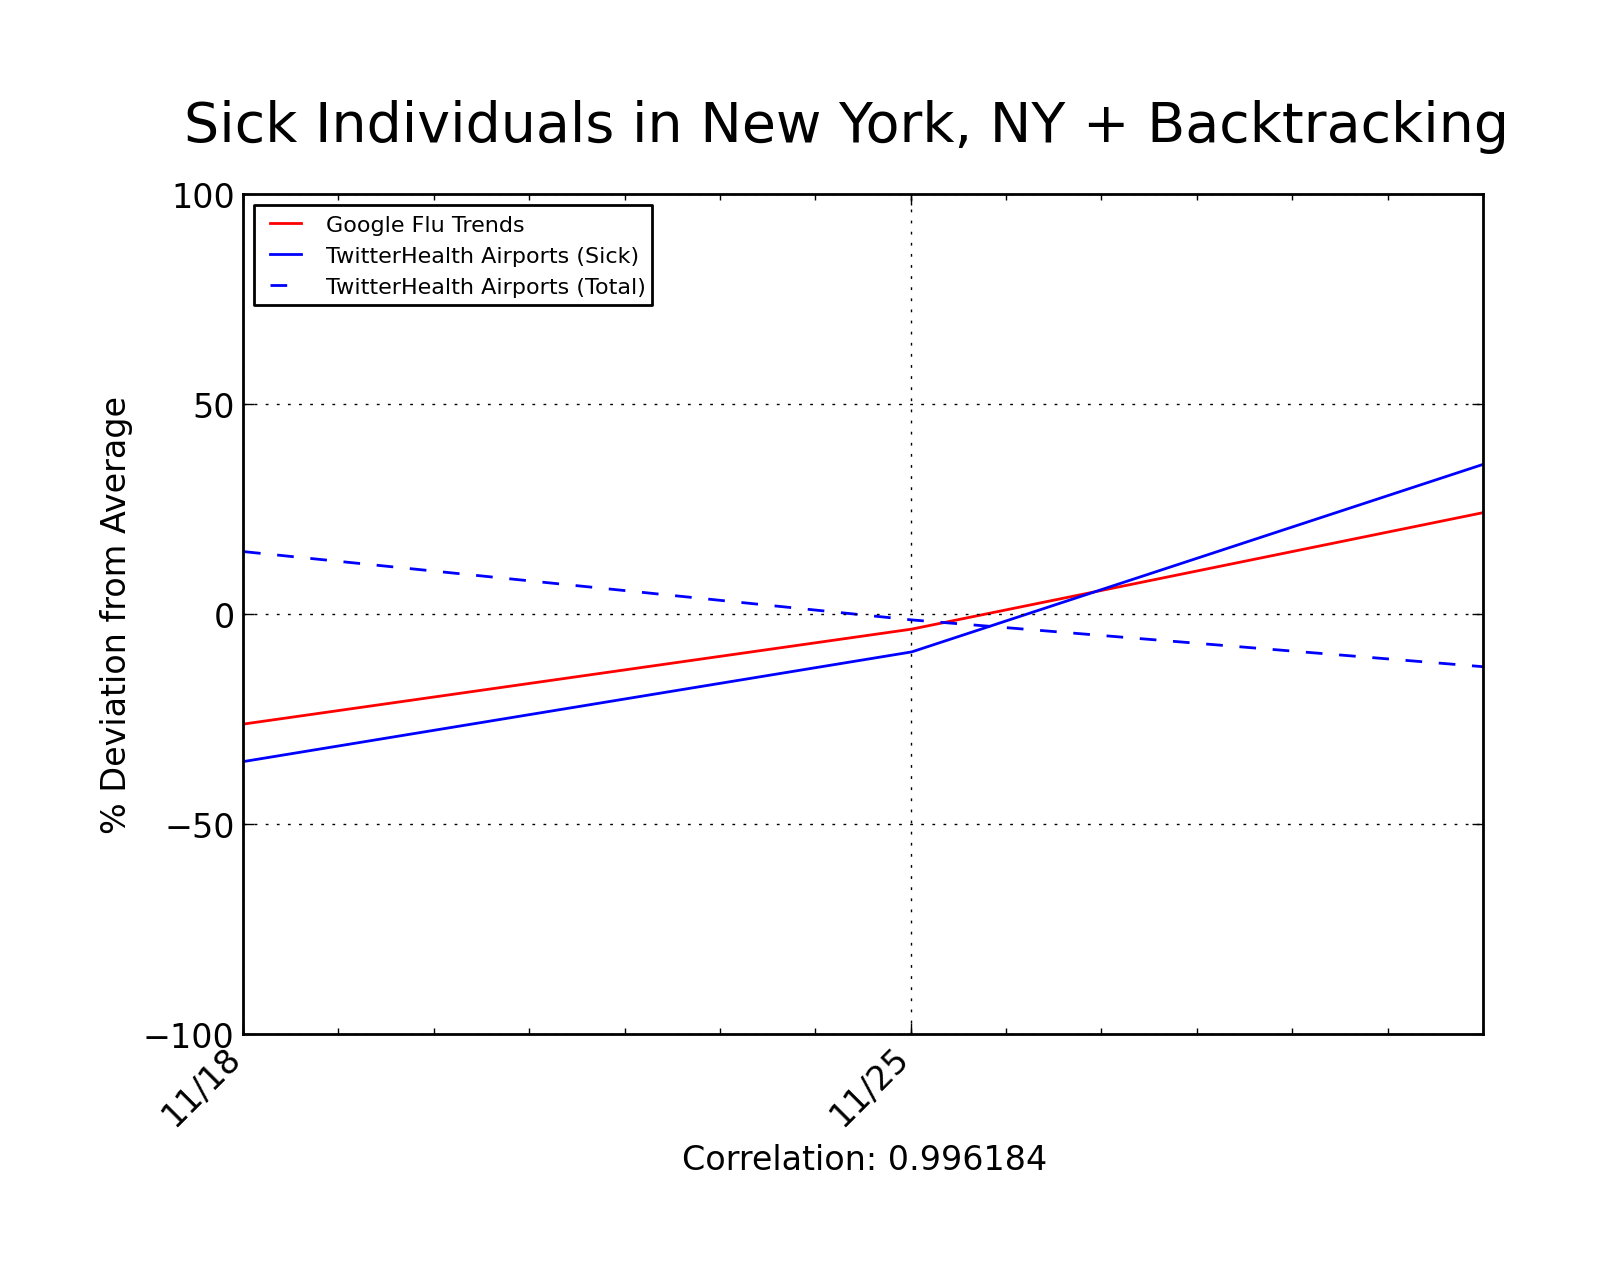
\includegraphics[width=\textwidth]{../plot/figures/JFK_idev_2012-12-16.png}
                    \end{subfigure}
                    \begin{subfigure}[t]{0.45\textwidth}
                        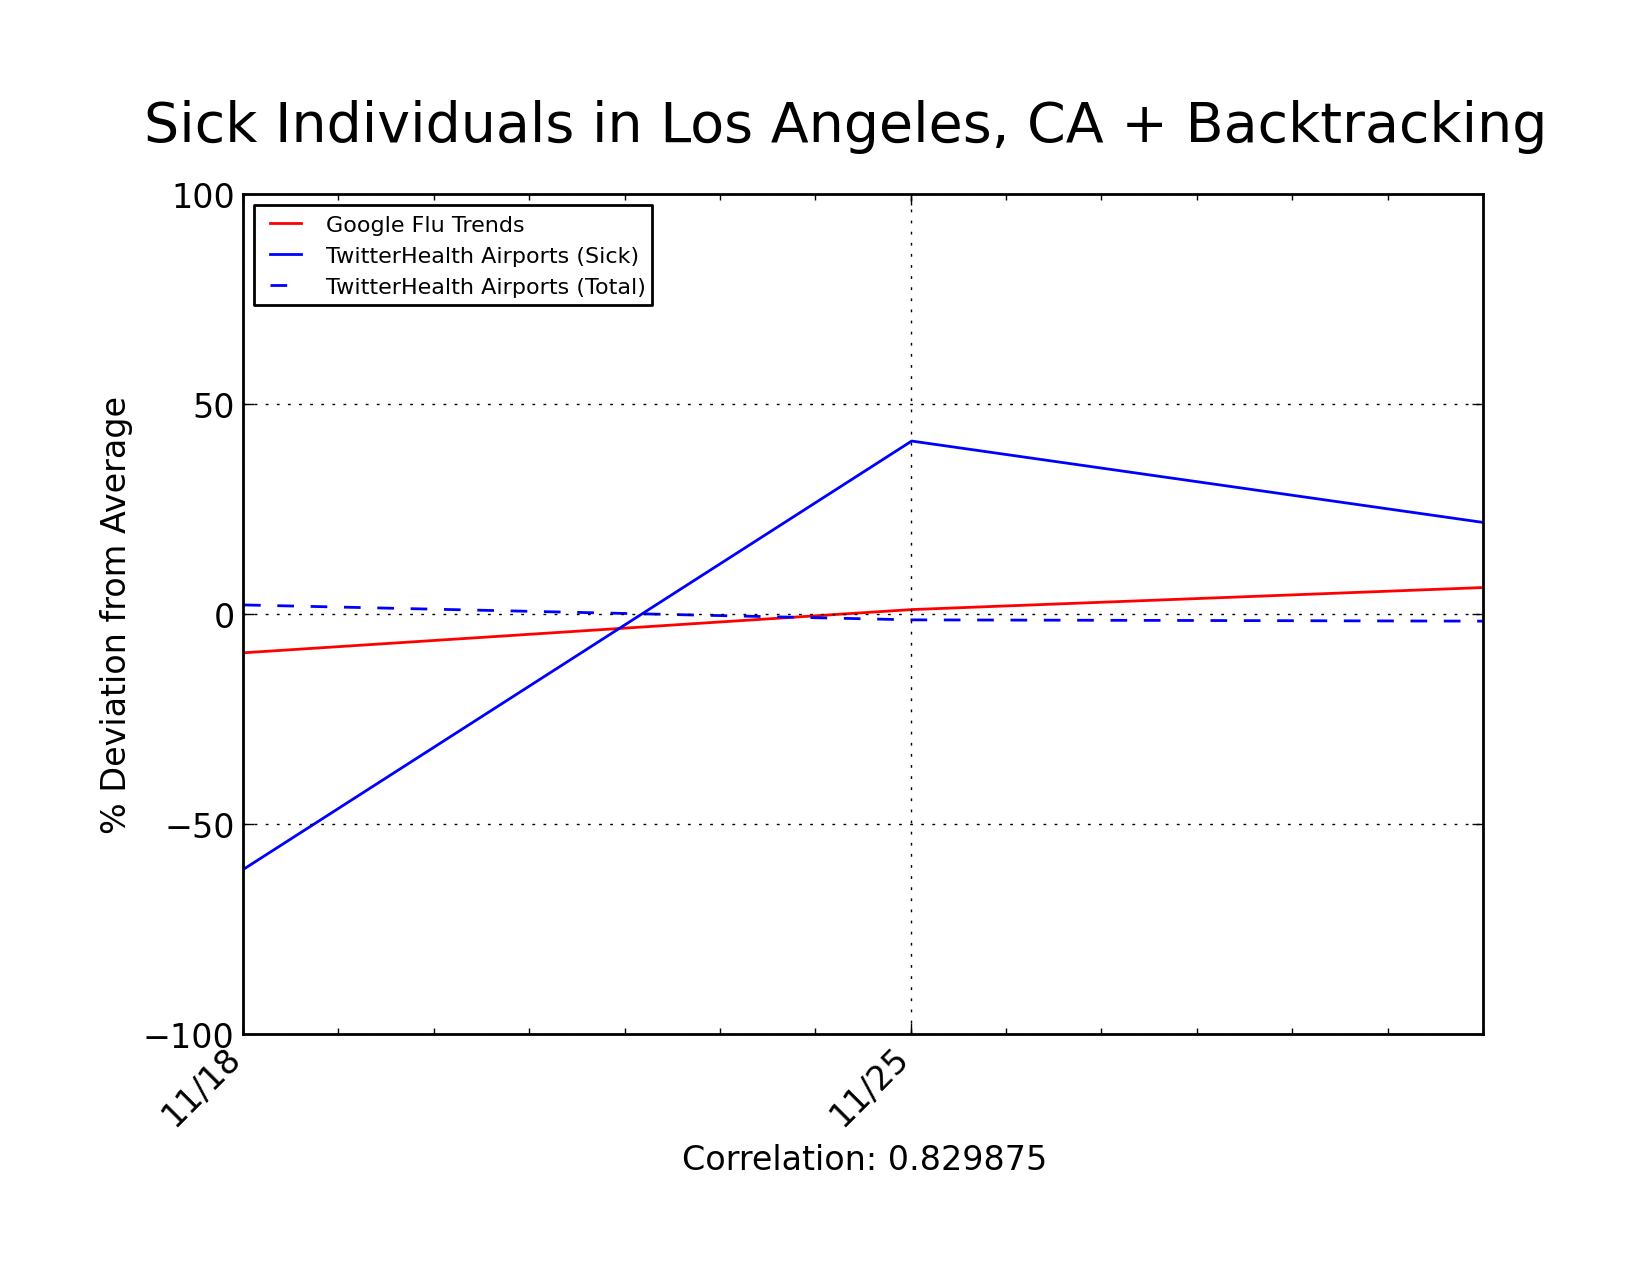
\includegraphics[width=\textwidth]{../plot/figures/LAX_idev_2012-12-17.png}
                    \end{subfigure}
                    \begin{subfigure}[b]{0.45\textwidth}
                        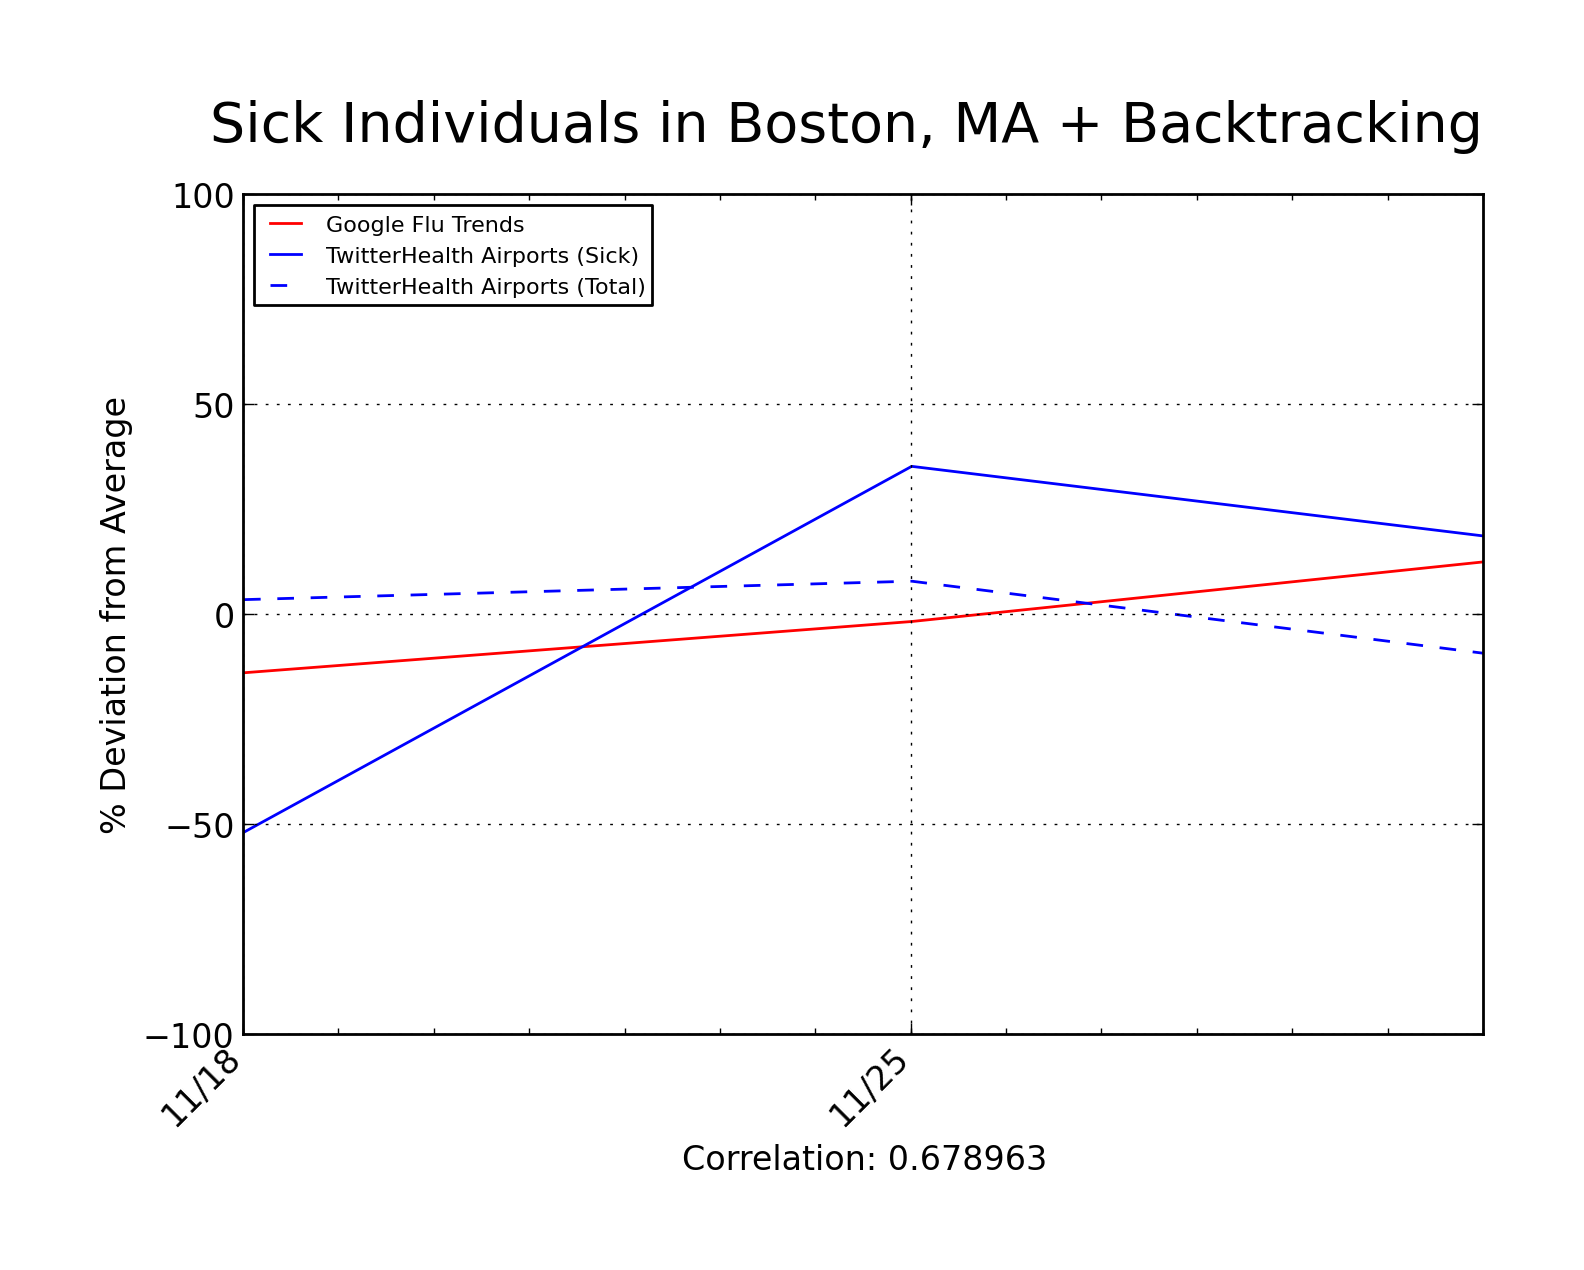
\includegraphics[width=\textwidth]{../plot/figures/BOS_idev_2012-12-17.png}
                    \end{subfigure}
                    \begin{subfigure}[b]{0.45\textwidth}
                        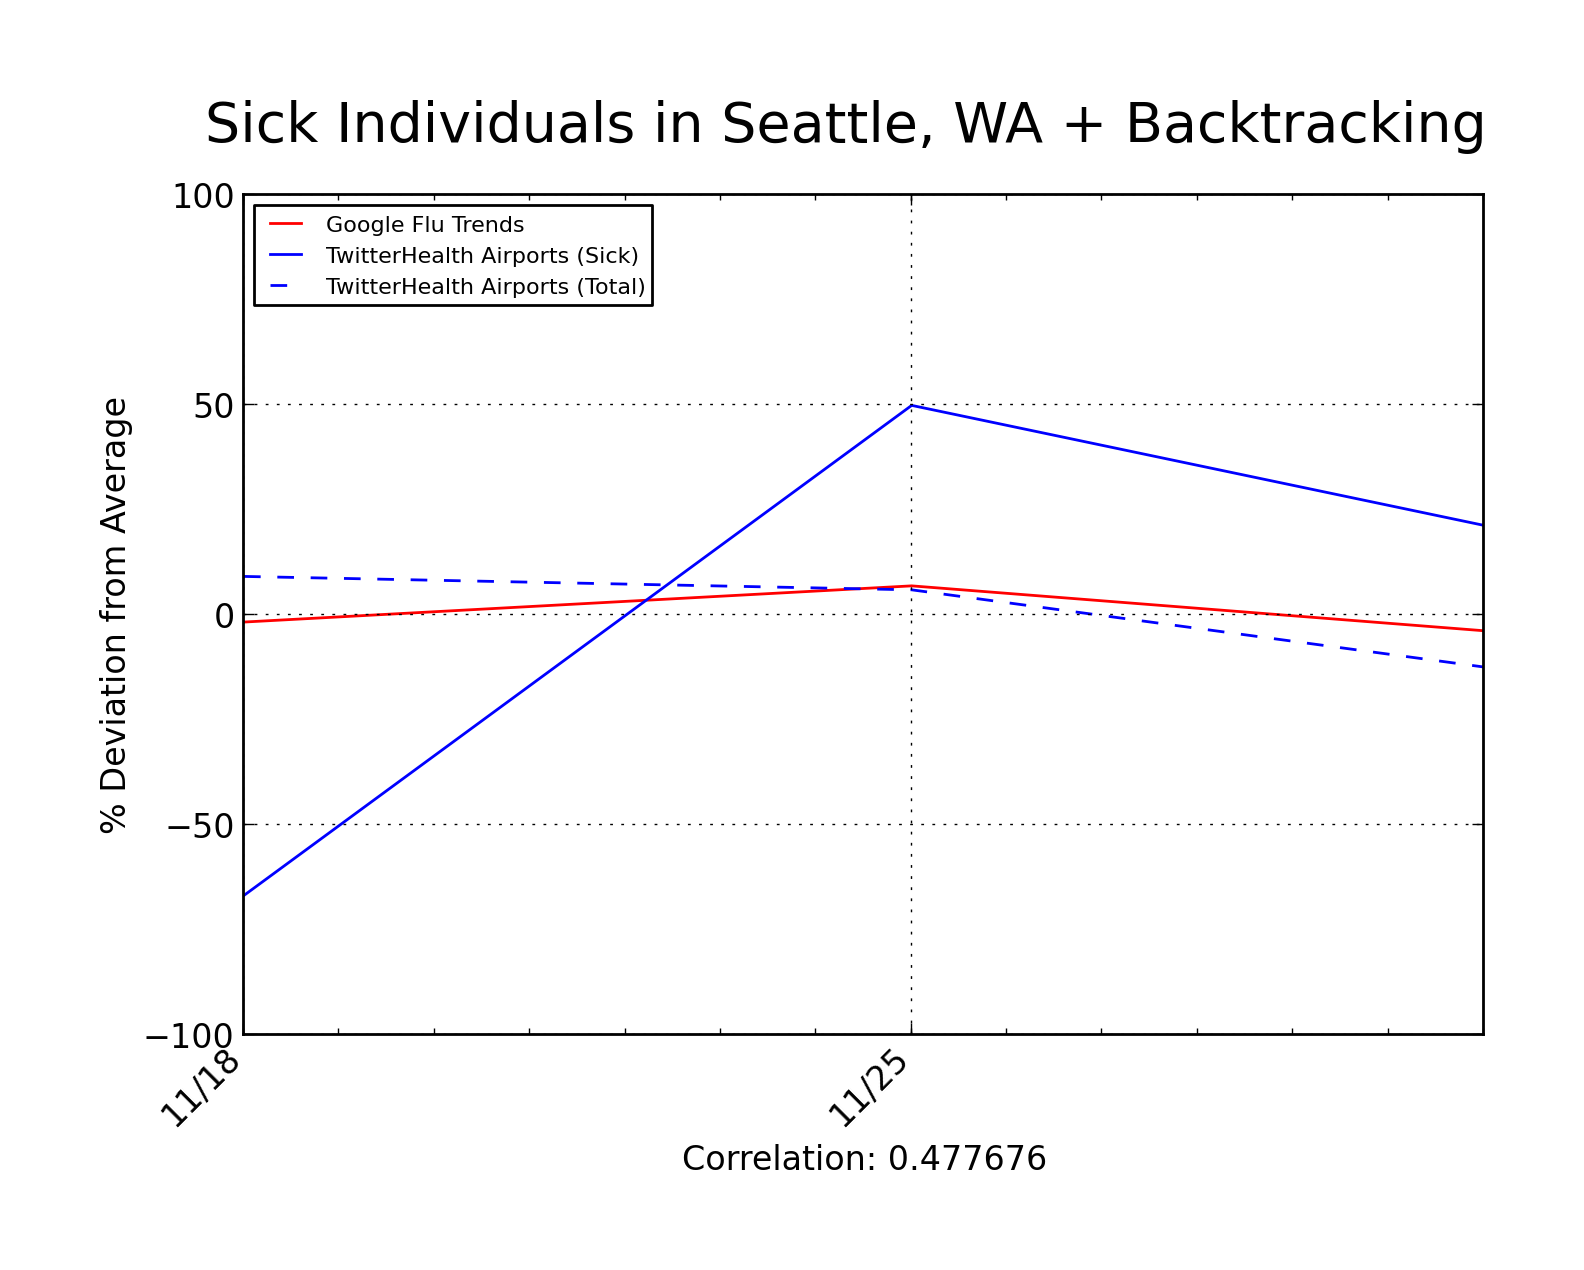
\includegraphics[width=\textwidth]{../plot/figures/SEA_idev_2012-12-16.png}
                    \end{subfigure}
                    \caption{Results from our airports dataset, and their correlations with Google Flu Trends data for the regions they serve.}
                    \label{backtrack-comparison}
                \end{center}
            \end{figure}

            After this initial analysis, we began to start examining how our novel systems compared to the official statistics. This process is tricky not only because of the execution time of some of our methods, which is considerable in some cases, but also because of the size of our datasets. Our data set is small in terms of simple volume: we simply don't have as many sick tweets made from airports as Google has Google searches related to influenza. It is also small in terms of time covered. We only started collecting for this project about three or four weeks ago, so we only have reasonably complete data for a month-long period. This pales in comparison to our previous projects, which have up to three months of data at this point.

            The result of the first factor is that our data is much more sensitive to smaller variations: a surge in maybe just ten sick people will lead to a spike of 200\% deviation from the mean for a small airport, for example, whereas a surge of even 100 cases of influenza in the Google Flu trends data is barely a blip on the radar. The result of the second factor is that measures of correlation are a lot more tenuous: there are fewer data points to consider, so minor differences tend to be exaggerated, and even the addition of one more data point could change the correlation coefficient dramatically.

            Despite these challenges, we applied the same analytic procedures I discussed in the previous section to our new techniques, specifically the backtracking of ``frequent flyers'' I mentioned in the Methodology section. The idea behind collecting timelines for these users is that we can easily observe which individuals are flying based on if they have tweeted from two or more airports, excepting cases such as bots, but it is very rare that these observations also come with strong health observations. The hope is that, by looking back in their timelines, we can find some strong health observation from within a couple of days of arriving at an airport, and from this infer that they are quite likely still sick when they get there.

            We were pleasantly surprised to find that using this backtracking did, in fact, increase the number of individuals identified as being sick. In Boston, for example, including backtracking nearly doubled the amount of sick people we found. But, of course, that's all worthless if that data doesn't match up with official stats. Even over our small time span, however, we found that our backtracking approach still correlated positively with Google Flu trends. You can see some of our results in Figure~\ref{backtrack-comparison}. There was much more variation in the correlation coefficients, with some regions being much stronger than in our previous analysis and some regions being much weaker. This was no doubt an effect of the small time interval, so we hope that having a couple more months will make these correlations less variable and stronger.

            Unfortunately, at this time we do not have results for our meetings model. This is not only the result of the collection time once again, but also the extreme delicacy and complexity of the meetings model. As previously discussed, there is a performance issue related to the number of users in the meetings model, so we are working on choosing some close-to-ideal set of active users in our dataset who have visited many airports that we can test over. Additionally, and unsurprisingly, there is also a great deal of parameter tweaking involved in the DBN model, so we will have to try out a few different configurations and see which gives the best results. We hope to have some preliminary results for this by the end of break.

        \subsection{Measuring Influx}
            While all this previous analysis is good and establishes the validity of our approach, we believe that the true power of our new model lies in its predictive capabilities. To this end, we have devised a method for analyzing the influx of sick individuals into a given airport or region, appropriately called \emph{disease influx}. Influx can be described by this equation:

            \[ I(t, x) = \frac{\sum_{i \in A \setminus x} sickFlying(t, i \rightarrow x)}{\frac{1}{|D|} \sum_{d \in D} \sum_{i \in A \setminus x} sickFlying(d, i \rightarrow x)} \]

            In essence, influx is a value proportional to the deviation of one day from the mean. It considers the number of sick people who have arrived at airport $x$ on day $t$ from all other airports. If a day is ``completely normal'', that is, the number of sick people arriving at that airport on that day was exactly the average, $I(t, x)$ will be $1.0$. Therefore, values below this indicate slightly less than average, and values above this indicate a larger volume of sick individuals.

            \begin{figure}[b!]
                \begin{center}
                    \includegraphics[width=1.0\textwidth]{/Users/soba/Desktop/influx-example.png}
                    \caption{Influx measures obtained over a nine day period on a small sample of our dataset.}
                    \label{influx-example}
                \end{center}
            \end{figure}

            The hope is that large spikes in the influx measure on a certain will correlate strongly with large spikes in influenza in that region a few days later. Based on some example cases we have worked through on samples of our data set, we have found that the influx on most days for most airports is 0.0 or some similarly small value, so increases in the volume of sick people tend to stick out. You can see an example of this in Figure~\ref{influx-example}.

            The implications of such a correlation would be enormous indeed: we would essentially be predicting illness trends days before they even happened. Such information could help public agencies target their efforts to regional health concerns in real-time rather than cast a wide net and hope they reach their audience at the right time. Furthermore, the aggregate influx can be easily decomposed to uncover which other airport was most responsible for the surge. Unfortunately, we will need much more data over a longer time period before we can even begin to analyze the validity of this measure.

    \section{Future Work}
        The most exciting thing about this project is the endless possibilities that branch off from this one. Here are just a couple that we have recently considered.

        \subsection{More Localized Meetings}
            Another obvious application of our meetings model is over much more localized areas, such as individual neighborhoods in cities. We have already done some exploratory work in this area, and it is actually where we originally got the idea for this airports branch of TwitterHealth. One advantage that this study has over airports is, with exception of things such as cars and subways, there is very little of the hyper-diffusive movement that complicates epidemiological models. Adam has also proposed an algorithm inspired by dendrogram-based hierarchical clustering methods to discover high-ranking individuals or venues that contribute most significantly to disease within these local populations. We are still working out the details of this approach.

        \subsection{More Detailed Flight Information}
            One possible deficiency of our meetings and influx models is that they do not make use of actual flight information, they just infer who has been flying based on their geotagged tweets. In this way, we assume that the locations you tweeted from were endpoints of a discrete and indivisible line segment. This is problematic if, for example, someone flew from Rochester to San Francisco with a connecting flight in Atlanta, and that person only tweeted in Atlanta and San Francisco. Unfortunately there's not a lot we can do about this case; however, if you were to have tweeted in Rochester instead of Atlanta, we could leverage some information about flights and layovers to infer that you were probably in Atlanta at some point in between. This could be incredibly useful, since we could be missing huge contributions to the influx of flu in Atlanta without it.
        
    \newpage
    \bibliographystyle{plain}
    \bibliography{citations}
\end{document}